\documentclass[border=3pt]{standalone}
\usepackage[utf8]{inputenc}
\usepackage[T1]{fontenc}
\usepackage{tikz}
\usetikzlibrary{arrows.meta,positioning,fit,backgrounds}
\begin{document}
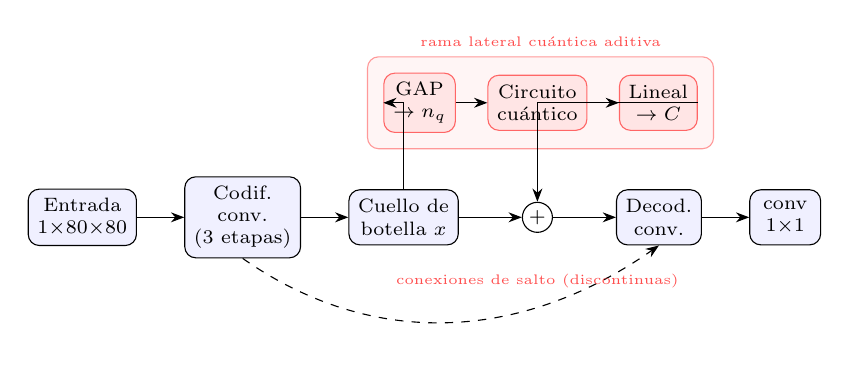
\begin{tikzpicture}[
  font=\scriptsize,
  box/.style={draw,rounded corners,minimum height=7mm,minimum width=9mm,align=center},
  qbox/.style={box,fill=red!10,draw=red!60},
  cbox/.style={box,fill=blue!6},
  >/.tip={Stealth},every edge/.style={draw,-Stealth}
]
\node[cbox] (in) {Entrada\\$1{\times}80{\times}80$};
\node[cbox,right=6mm of in] (enc) {Codif.\\conv.\\(3 etapas)};
\node[cbox,right=6mm of enc] (bn) {Cuello de\\botella $x$};
\node[circle,draw,inner sep=1pt,right=8mm of bn] (add) {$+$};
\node[cbox,right=8mm of add] (dec) {Decod.\\conv.};
\node[cbox,right=6mm of dec] (head) {conv\\$1{\times}1$};
\node[qbox,above=9mm of add] (qc) {Circuito\\cuántico};
\node[qbox,left=4mm of qc] (gap) {GAP\\$\to n_q$};
\node[qbox,right=4mm of qc] (po) {Lineal\\$\to C$};
\draw (in) edge (enc);
\draw (enc) edge (bn);
\draw (bn) edge (add);
\draw (add) edge (dec);
\draw (dec) edge (head);
\draw[-Stealth] (bn.north) |- (gap.west);
\draw (gap) edge (qc);
\draw (qc) edge (po);
\draw[-Stealth] (po.east) -| (add.north);
\draw[dashed,-Stealth] (enc.south) to[out=-35,in=-145] (dec.south);
\node[font=\tiny,below=4mm of add,red!70] {conexiones de salto (discontinuas)};
\begin{scope}[on background layer]
\node[draw=red!40,rounded corners,fill=red!4,fit=(gap)(qc)(po),inner sep=2mm,
  label={[red!70,font=\tiny]above:rama lateral cuántica aditiva}] {};
\end{scope}
\end{tikzpicture}
\end{document}
